%
% tetraeder.tex
%
% (c) 2021 Prof Dr Andreas Müller, OST Ostschweizer Fachhochschule
%
\documentclass[tikz]{standalone}
\usepackage{times}
\usepackage{amsmath}
\usepackage{txfonts}
\usepackage[utf8]{inputenc}
\usepackage{graphics}
\usetikzlibrary{arrows,intersections,math,calc}
\usepackage{ifthen}
\begin{document}

\newboolean{showgrid}
\setboolean{showgrid}{false}
\def\breite{7}
\def\hoehe{4}

\begin{tikzpicture}[>=latex,thick]

% Povray Bild
\node at (0,0) {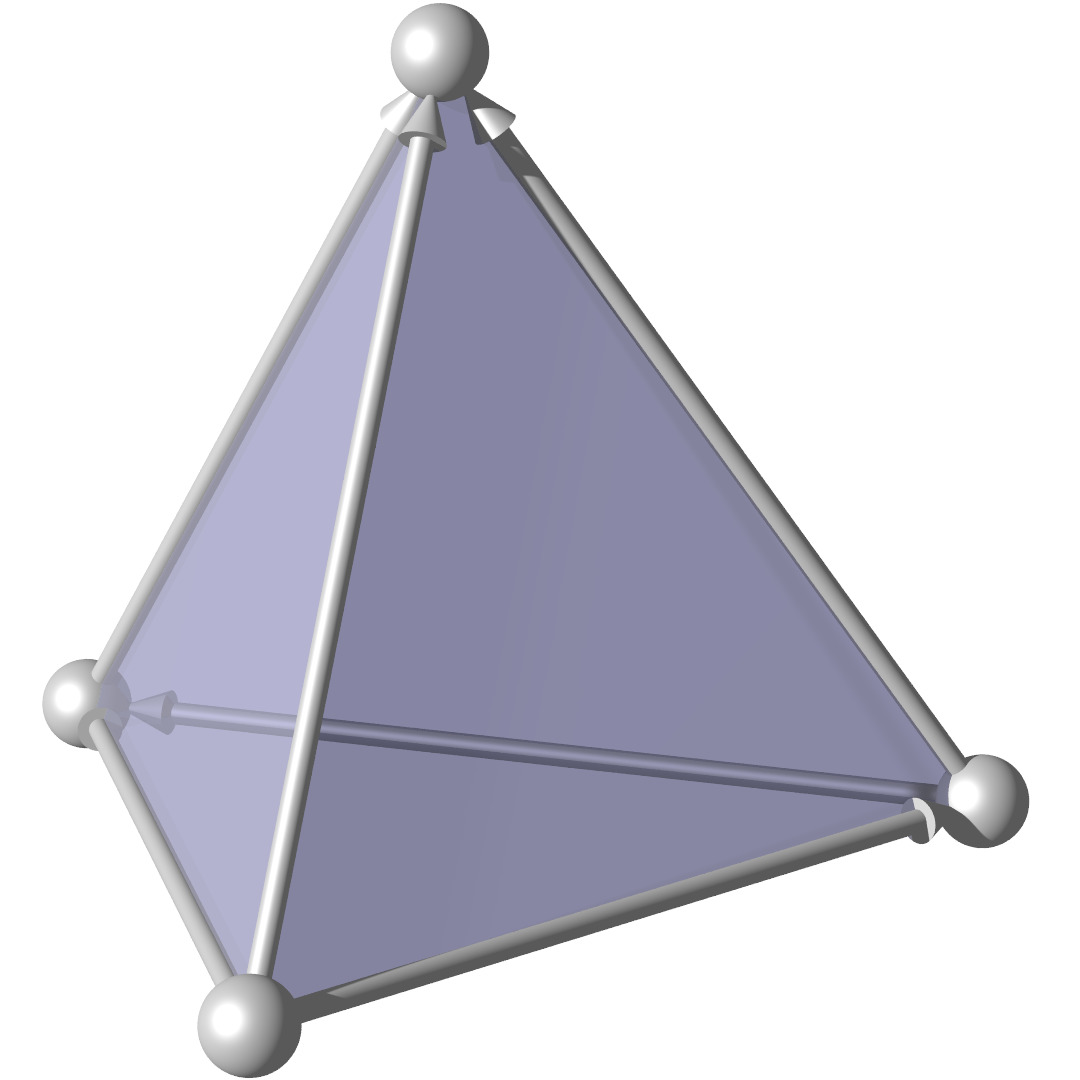
\includegraphics[width=8cm]{tetraeder.jpg}};

% Gitter
\ifthenelse{\boolean{showgrid}}{
\draw[step=0.1,line width=0.1pt] (-\breite,-\hoehe) grid (\breite, \hoehe);
\draw[step=0.5,line width=0.4pt] (-\breite,-\hoehe) grid (\breite, \hoehe);
\draw                            (-\breite,-\hoehe) grid (\breite, \hoehe);
\fill (0,0) circle[radius=0.05];
}{}

\def\knoten#1#2{
	%\fill[color=white,opacity=0.5] #1 circle[radius=0.2];
	\node at #1 {$#2$};
}

\knoten{(-2.2,-3.6)}{0};
\knoten{( 3.3,-1.9)}{1};
\knoten{(-3.4,-1.2)}{2};
\knoten{(-0.75,3.6)}{3};

\def\s{0.2}

\def\kante#1#2{
	%\fill[color=white,opacity=0.5] #1 circle[radius=0.2];
	\fill[color=white,opacity=0.5] 
		($#1+(-\s,-\s)$) --
		($#1+(+\s,-\s)$) --
		($#1+(+\s,+\s)$) --
		($#1+(-\s,+\s)$) -- cycle;
	\node at #1 {$#2$};
}

\kante{(0.5,-2.8)}{k_0}
\kante{(-2.8,-2.3)}{k_1}
\kante{(-1.4,0)}{k_2}
\kante{(-0.4,-1.55)}{k_3}
\kante{(1.25,0.95)}{k_4}
\kante{(-2.08,1.1)}{k_5}

\def\r{0.33}

\def\flaeche#1#2{
	\fill[color=white,opacity=0.5]
		($#1+({-\r*cos(30)},{-\r*sin(30)})$) --
		($#1+({\r*cos(30)},{-\r*sin(30)})$) --
		($#1+(0,{\r})$) -- cycle;
	\node at #1 {$#2$};
}

\flaeche{(-0.7,-5)}{f_0}
\draw (-0.7,-4.7) -- (-0.7,-3.25);
\draw[->,color=black!70] (-0.7,-3.06) -- (-0.7,-2.5);
\flaeche{(0.2,-0.5)}{f_1}
\flaeche{(-2.3,-0.7)}{f_2}
\coordinate (A) at (1,2.6);
\coordinate (B) at (0,1);

\flaeche{($1.2*(A)-0.2*(B)$)}{f_3}

\def\t{0.58}
\pgfmathparse{1-\t}
\xdef\T{\pgfmathresult}
\draw (A) -- ($\t*(A)+\T*(B)$);

\def\t{0.48}
\pgfmathparse{1-\t}
\xdef\T{\pgfmathresult}
\draw[->,color=black!70] ($\t*(A)+\T*(B)$) -- (B);


\end{tikzpicture}

\end{document}

